% typ dokumentu
\documentclass[12pt,twoside]{article}

% użycie pakietu , jak include
\usepackage{weiiszablon}

% autor pracy
\author{Krystian Olszowy}

% np. EF-123456, EN-654321, ..., Numer albumu
\studentID{EA-167582}

\title{Tworzenie drzewa składniowego języka ST}
\titleEN{{Creating an ST language syntax tree}}


%%% wybierz rodzaj pracy wpisując jeden z poniższych numerów: ...
% 1 = inżynierska	% BSc
% 2 = magisterska	% MSc
% 3 = doktorska		% PhD
%%% na miejsce zera w linijce poniżej
\newcommand{\rodzajPracyNo}{2}


%%% promotor
\supervisor{dr inż. Jan Sadolewski}
%% przykład: dr hab. inż. Józef Nowak, prof. PRz

%%% promotor ze stopniami naukowymi po angielsku
\supervisorEN{Jan Sadolewski, PhD, Eng.}


%% DO ZROBIENIA %%
\abstract{Praca zawiera zaproponowane rozwiązanie sterowania telewizorem z poziomu smartfona dzięki aplikacji mobilnej i urządzeniu pośredniczącemu, opartemu o mikrokontroler z niezbędnymi modułami. Przedstawiono i omówiono w niej technologie i koncepty, z których korzystano podczas procesu projektowania i tworzenia rozwiązania. Opisane zostały też najważniejsze elementy fizycznej części systemu, oprogramowanie mikrokontrolera, zbudowana aplikacja mobilna oraz ich współpraca w celu sterowania urządzeniem telewizyjnym.}
\abstractEN{The work encompasses a solution for television control through a smartphone application and an intermediary device, based on a microcontroller with necessary modules. It introduces and discusses the technologies and concepts employed during the design and building process. Additionally, it details the key components of the physical system, microcontroller software, the developed mobile application, and their collaboration for television device control.}

%% DO ZROBIENIA %%
\keywords{ST language, syntax tree, CPDev, Flutter, aplikacja mobilna}
\keywordsEN{remote controller, BLE, IR, Flutter, mobile application}


\begin{document}

% strona tytułowa
\maketitle

\blankpage

% spis treści
\tableofcontents

\clearpage
\blankpage

\section{Wstęp}
\subsection{Zintegrowane środowiska programistyczne (ang. IDE)}
Współczesny inżynier czy programista automatyki nie wyobraża sobie pracy bez dostępu do zintegrowanego środowiska programistycznego (ang. IDE). Środowiska te, będące podstawowym narzędziem w pracy twórców oprogramowania sterowników PLC, przekształciły się z prostych edytorów kodu w zaawansowane platformy wspierające projektowanie, symulację, testowanie i wdrażanie systemów sterowania. Dzięki nim możliwe jest nie tylko wygodne tworzenie logiki sterującej, ale również wizualizacja procesów, zarządzanie konfiguracją sprzętu czy analizowanie działania programu w~czasie rzeczywistym.

Na rynku dostępnych jest wiele rozwiązań, różniących się zakresem funkcji, kompatybilnością z określonymi typami sterowników oraz poziomem zaawansowania użytkownika. Jednym z przykładów takiego środowiska jest CPDev - polskie oprogramowanie tworzone na Politechnice Rzeszowskiej wspierające języki programowania zgodne z normą IEC 61131-3, które umożliwia programowanie sterowników różnych producentów, symulację działania programu oraz jego późniejsze wdrożenie na urządzeniu docelowym. Choć wiele firm korzysta z komercyjnych środowisk oferowanych przez producentów sterowników, takich jak TIA Portal czy GX Works, to rosnąca popularność rozwiązań niezależnych - jak CPDev - pokazuje, że możliwe jest tworzenie otwartych, elastycznych i konkurencyjnych narzędzi dla branży automatyki.

\subsection{Drzewa składniowe}
Drzewa składniowe to jedno z tych narzędzi, które trudno przecenić w świecie programowania. Choć na pierwszy rzut oka mogą wydawać się technicznym detalem, w~praktyce są fundamentem działania wielu elementów środowisk programistycznych. To właśnie one przedstawiają kod w postaci uporządkowanej struktury, zgodnej z gramatyką danego języka, dzięki czemu program może być łatwiej analizowany i przetwarzany.

Bez drzew składniowych trudno wyobrazić sobie działanie kompilatorów, interpreterów, a nawet tak podstawowych funkcji edytora jak kolorowanie składni, podpowiadanie składniowe czy automatyczne formatowanie kodu. Dzisiejsze IDE bazują na tych strukturach niemal na każdym kroku - to one pozwalają na bieżąco wykrywać błędy w kodzie, usprawniają nawigację po projekcie i umożliwiają wprowadzenie inteligentnych podpowiedzi.

Automatyczne generowanie parserów, znacząco przyspiesza cały proces. Programista nie musi już ręcznie tworzyć złożonych analizatorów składni, co oszczędza czas i~ogranicza liczbę błędów.

Dla środowiska CPDev możliwość wygenerowania drzewa składniowego dla języka ST to istotne ułatwienie. Dzięki temu można nie tylko szybciej i prościej zaimplementować parser zgodny z normą IEC 61131-3, ale też stworzyć solidną podstawę do rozwijania edytora o nowe funkcje - jak choćby inteligentne podpowiedzi, analiza semantyczna czy lepsza diagnostyka błędów. To wszystko przekłada się na wygodniejszą pracę użytkownika i otwiera drogę do dalszego rozwoju CPDeva jako nowoczesnego narzędzia do programowania sterowników.


\subsection{Cel pracy}
Celem pracy jest przygotowanie interpretera kodu generującego drzewo składniowe języka ST zgodnego z normą IEC 61131-3 oraz oprogramowaniem CPDev, na~podstawie podanego kodu źródłowego tego języka. Oprogramowanie generujące drzewo składniowe ma współpracować z kodem w języku C\#. Aby takie oprogramowanie przygotować, należy wcześniej także przeprowadzić badanie porównawcze narzędzi do tworzenia drzew składni języków formalnych opisanych za pomocą gramatyki bezkontekstowej i wybrać rozwiązanie najbardziej odpowiadające postawionemu zadaniu.

\subsection{Zakres pracy}
Zakres pracy obejmuje prównanie wybranych narzędzi do tworzenia drzew skła\-dni języków formalnych opisanych za pomocą gramatyki bezkontekstowej i wybranie najlepszego z nich do interpretowania języka ST zgodnego z normą IEC 61131-3 w~CPDevie. Praca podejmuje także tematykę utworzenia pliku gramatyki języka ST dla najbardziej odpowiedniego z analizowanych narzędzi i przetestowania wygenerowanego oprogramowania dla przykładowych kodów źródłowych.


\subsection{Zawartość pracy DO ZROBIENIA}
W rozdziale drugim  omówiono ogólnodostępne rozwiązania stanowiące aktualny stan wiedzy w zakresie zdalnego sterowania odbiornikiem telewizyjnym. Prównano je z autorskim systemem wskazując jego zalety i rozwiązywane przez niego problemy.

Rozdział trzeci zawiera przedstawienie i opis technologii wykorzystanych w zaprojektowanym rozwiązaniu. Są to: Platforma ESP32, język programowania C++, framework Arduino, podczerwień, system Android, język programowania Dart, framework Flutter oraz techonlogia Bluetooth Low Energy.

Czwarty rozdział opisuje sposób połączenia komponentów składających się na urządzenie pośredniczące zbudowane aby skomunikować aplikację mobilną z telewizorem. Zawarte zostały w nim także opisane scharakteryzowane parametry tych komponentów.

W rozdziale piątym szczegółowo omówiono utworzone oprogramowanie mikrokontrolera odpowiedzialne za sterowanie jego zasobami i dołączonymi modułami fizyczymi. Przedstawione zostały ważniejsze kody źródłowe projektu oraz ich działanie.

Rozdział szósty zawiera opis zaprojektowanego intefejsu użytkownika aplikacji mobilnej oraz jej funkcjonalności. Ukazane zostały także wykorzystane podczas implementacji, rozwiązania programowe.

Siódmy rozdział koncentruje się na przedstawieniu sposobu korzystania z utworzonego rozwiązania. Dokonywana jest także ocena skuteczności działania poszczególnych funkcji systemu.

W ostatnim rozdziale zawarto podsumowanie całej pracy, możliwe usprawnienia zaprojektowanego rozwiązania. Wskazane zostały też elementy projektu, które autor uważa za wkład własny.


\clearpage
\section{Przedstawienie oprogramowania CPDev}
\subsection{Omówienie dostępnych rozwiązań}
Na rynku można znaleźć niezliczoną ilość pilotów uniwersalnych. Rożnią się one
ceną, obsługiwanymi funkcjonalnościami czy sposobami zasilania. Większość z nich zazwyczaj
wykorzystuje programowanie przycisków oparte na nasłuchiwaniu sygnałów podczerwonych z pilota, co dla niektórych użytkowników może stanowić
wyzwanie, ze względu na uciążliwą obsługę procesu i znikomą informację z pilota o powodzeniu odebrania sygnału. Cena rzędu jedynie kilku czy kilkunastu złotych
,już na polskim rynku, kusi jednak potencjalnych nabywców, nawet pomimo wątpliwej jakości wykonania. Przykładem
takiego pilota uniwersalnego może być urządzenie Interlook L336\cite{cheapController}.

Więksi producenci oferują również piloty uniwersalne z predefinowanymi sygnałami dla przycisków. Jednak,
prawie zawsze są to grupy przycisków z modeli właśnie tego producenta. Uwadze nie umyka także wyższa cena takich
rozwiązań argumentowana zazwyczaj prestiżem marki i jakością wykonania. Takie rozwiązanie znaleźć
możemy na przykład w modelu Philips SRP4030/10\cite{expensiveController}.

Dostępne są jednak także rozbudowane aplikacje z dedykowanymi urządzeniami wysyłającymi sygnały podczerwone łączące się ze smartfonem poprzez WiFi. Znajdujemy już w nich wiele z pożądanych cech w pilocie uniwersalnym, jak możliwość otrzymania predefiniowanych modeli telewizorów czy edycję nie wymagającą posiadania oryginalnego pilota do sterowanego urządzenia. Przykładowym dostępnym rozwiązaniem tego typu jest urządzenie Smart IR Remote Crabtree\cite{appController}.
\subsection{Zestawienie z autorskim projektem}
{Wymienione wcześniej urządzenia mają swoje zastosowania, ale nie wystrzegają się też wad. Wiele z nich wymaga zasilania bateryjnego, co jest szkodliwe dla środowiska, o które, szczególnie stara się dbać społeczeństwo w dzisiejszych czasach. Posiadają one często mozolne i łatwe w popełnieniu błędu programowanie. Dostęp do tworzenia własnych zestawów przycisków jest nierzadko trudny, czasem niemożliwy, a samo użycie często wymaga przchodzenia po niewidocznej liście i sprawdzeniu czy telewizor reaguje na predefiniowane przyciski. Urządzenia nieposiadające tych wad czyli aplikacje z dedykowaną stacją wysyłającą sterowanie do urządzeń domowych, łączą się jednak poprzez WiFi ze smartfonem, przez co pobierają więcej energii niż inne rozwiązania oraz wymagają podłączenia do sieci użytkownika, generując jej obciążenie.

Autorskie rozwiązanie systemu służacego za pilota do telewizora stara się rozwiązać przedstawione problemy. Bateria czy akumulator możliwe są do używania z~urządzeniem wysyłającym sygnały podczerwone, jednak z powodzeniem zasilanie może i~powinno odbywać się przez kabel microUSB, dzięki czemu nie zwiększany jest popyt na szkodliwe dla środowiska baterie. Programowanie przycisków odbywa się przez podanie kodów IR w odpowiednich polach, które sprawdzają czy dane w nich zawarte są poprawne, dzięki czemu użytkownik ma bezpośredni i przejrzysty dostęp do swoich ustawień pilota. Utworzony przez niego lub predefiniowany model telewizora wybierany jest z listy, którą można łatwo przeglądać i rozbudować. Sama aplikacja posiada kontrolę błędów konfiguracji oraz komunikacji bezprzewodowej i jest intuicyjna dla użytkownika już podczas pierwszego uruchomienia. Wymiana danych ze smartfonem odbywa się za pomocą technologii Bluetooth Low Energy co ogranicza zużycie energii. Zauważając, że z urządzenia pośredniczącego może korzystać wiele osób jednocześnie w większej skali jest to tańsze rozwiązanie niż piloty uniwersalne. Dodatkowo łatwość obsługi i przejrzystość interfejsu, które zapewnia aplikacja są atutami tego rozwiązania zwłaszcza dla osób starszych, nieobytych z technologią.
}
\clearpage
\section{Przedstawienie wykorzystanych technologii}
\subsection{Platforma ESP32}
ESP32 jest układem typu SoC (ang. System-on-a-chip) produkowanym przez chińską firmę Espressif Systems,
wyposażony jest najczęściej w dwurdzeniowy procesor Xtensa LX6 o taktowaniu 240 MHz\cite{esp32Datasheet}. W większości przypadków podczas rozwijania projektu używany jest będąc osadzonym na płytce deweloperskiej różnych producentów, co znacznie przyspiesza projektowanie i prototypowanie rzeczywistego systemu. Na rynku znajduje sie niezliczona ilość różnych wersji płytek deweloperskich przez co dopasowanie
jej do własnych potrzeb jest dużo łatwiejsze niż w przypadku innych rozwiązań. Przykładem takiej płytki, która została też użyta w projekcie, jest DOIT DevKit V1\cite{doitDevKitV1}. Na rysunku \ref*{Fig:devkitScheme} przedstawiono poglądowy shemat wyprowadzeń tej płytki deweloperskiej.

\begin{figure}[ht]
   \centering
   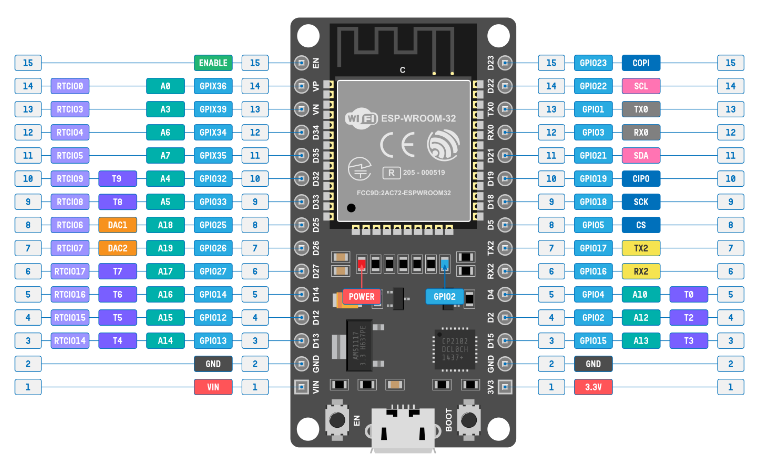
\includegraphics[width=13cm]{images/doit_devkit_v1.png}
   \caption{Schemat wyprowadzeń płytki DOIT DevKit V1 \cite{doitDevKitV1}}
   \label{Fig:devkitScheme}
\end{figure}

Jednym z kluczowych atutów platformy ESP32 jest wbudowane wsparcie dla Wi-Fi(802.11 b/g/n) i Bluetooth(klasyczny 4.2 i BLE), co umożliwia łatwe połączenie z siecią bezprzewodową oraz sprawną komunikację między urządzeniami zewnętrznymi.
Duża licz\-ba portów wejścia/wyjścia czyni go idealnym do obsługi wielu czujników, akscesoriów i modułów. Układ zawiera także zintegrowany konwerter analogowo-cyfrowy (ADC) umożliwiając precyzyjny pomiar sygnałów analogowych. System zawiera wiele innych możliwości, ale najważniejsze jego funkcjonalości i charakterystyczne cechy, firma Espressif zebrała na digramie,  który znalazł się na rysunku \ref*{Fig:functionalDiagram}.

\begin{figure}[ht]
   \centering
   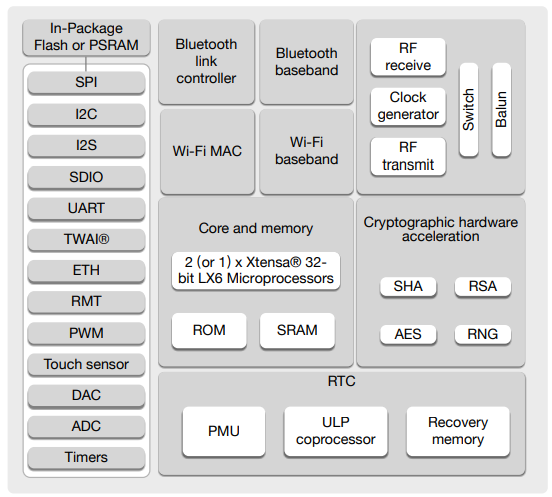
\includegraphics[width=12cm]{images/esp32_functional_diagram.png}
   \caption{Diagram funkcjonalności zaczerpnięty z dokumentacji techniczej ESP32\cite{esp32Datasheet}}
   \label{Fig:functionalDiagram}
\end{figure}

ESP32 został zoptymalizowany pod kątem efektywnego zużycia energii, co sprawia, że jest bardzo dobrym
wyborem dla aplikacji zasilanych bateryjnie lub kiedy ważny jest niski pobór prądu projektowanego systemu. Jego wszechstronność objawia
się obsługą przeróżnych protokołów komunikacji przewodowej,
takich jak SPI, I2C, UART, co sprawia, że integrację z zewnętrznymi modułami i systemami, można przeprowadzić w szybki i dostosowany do konkretnego przypadku sposób.

Warto podkreślić, że ESP32 cieszy się uznaniem wśród deweloperów, co przekłada się na dostęp do obszernej dokumentacji oraz wsparcie online na forach użytkowników. Programowalność w języku Arduino oraz możliwość korzystania
z MicroPython dodatkowo zwiększają elastyczność platformy, umożliwiając dostosowanie do indywidualnych potrzeb projektu.
Nieocenione są także biblioteki i moduły tworzone przez społeczność i udostępniane w formie otwartoźródłowej.
\subsection{Język programowania C++}
C++ jest językiem programowania, który swoje zastosowanie znalazł w wielu dziedzinach, gdzie ceni się wydajność rozwiązania. Mimo tego, że powstał w latach 80-dziesiątych na podstawie języka C, jego najnowsze wersje zdecydowanie można zaliczyć do nowoczesnych języków programowania.

Język ten jest kompilowany oraz stosuje silne typowanie statyczne, dzięki czemu, wykrywanie błędów na etapie tworzenia kodu jest znacznie łatwiejsze niż w przypadku innych podejść tworzenia programu wynikowego. Charakteryzuje się on także niskopoziomowym dostępem do pamięci, jak i możliwością jej dynamicznej alokacji w trakcie trwania programu, co zapewnia elastyczność implementacji i wysoką wydajność. C++ daje także możliwość korzystania z specyfikatora inline, który użyty dla funkcji powoduje, że kompilator kopiuje jej kod w zadane miejsce, zamiast umieszczać tam wkaźnik do niej. Przekłada się to na minimalizację narzutu czasowego związanego z wywołaniami bloków funkcyjnych. Język ten umożliwia także stosowanie podejścia obiektowego do projektowania oprogramowania, co z kolei sprzyja modularności rozwiązania i łatwości utrzymania kodu\cite{cppBjarne}.

Wydajność i możliwość niskopoziomowej kotroli zasobów urządzenia powoduje, że język ten jest  najczęściej używany do programowania skomplikownych gier
komputerowych, protokołów komunikacyjnych oraz systemów wbudowanych. Przez jego popularność dla systemów osadzonych, powstało wiele współracujacych z nim frameworków i bibliotek do obsługi rozmaitych mikrokontrolerów. Dzięki temu wybierając C++ jako język tworzenia oprogramowania systemu wbudowanego zyskuje się bardzo dużą kontrolę nad sprzętem oraz elastyczność w doborze narzędzi deweloperskich.

\subsection{Framework Arduino}
Framework Arduino to otwarte oprogramowanie, które umożliwia łatwe tworzenie aplikacji dla mikrokontrolerów zgodnych z standardem płytek Arduino. Bazuje na języku programowania C++ oraz wykorzystuje uproszczoną warstwę abstrakcji, co sprawia, że jest przyjazny dla początkujących, jednocześnie oferując zaawansowane funkcje dla doświadczonych programistów\cite{arduinoIntroduction}.

Framework oferuje prostą obsługę wejścia/wyjścia (I/O), dzięki czemu integracja z czujnikami, przekaźnikami i wieloma innymi modułami jest błyskawiczna i intuicyjna. Ponadto, zapewnia prosty sposób dostęp do interfejsów komunikacyjnych,
takich jak UART, SPI czy I2C. Ważną częścią frameworka Arduino są też przyjazne w~użyciu biblioteki tworzone także przez użytkowników, przez co niemal zawsze znajdzie się kod obsługujący żądaną funkcjonalność. Obejmują one obszar komunikacji bezprzewodowej, obsługi czujników, sterowania silnikami, czy obsługi ekranów LCD i OLED. Każde z nich są regularnie poprawiane przez firmę lub społeczność, dzięki czemu oprogramowanie staje się szybko aktualne i wspiera nowo dodane urządzenia i~narzędzia.
\subsection{Komunikacja za pomocą podczerwieni}
Komunikacja poprzez podczerwień\cite{infrared} (IR - Infra-Red) to forma przesyłania danych, wykorzystująca fale elektromagnetyczne
o niższej częstotliwości niż światło widzialne. Fale podczerwone znajdują się w zakresie elektromagnetycznym
poniżej czerwonego końca widma światła widzialnego, typowo w~zakresie od 300 GHz do 400 THz. Te fale są
niewidoczne dla ludzkiego oka, ale mogą być wykrywane i generowane przez diody. Typowo
wysyłając sygnał według konkretnego protokołu moduluje się go według określonego kodu liczbowego.
Modulacja może obejmować zmianę amplitudy, częstotliwości lub fazy fali podczerwonej. Gdy sygnał dociera do odbiornika
(zazwyczaj zasięg komunikacji wynosi do 10m), odbiornik wyposażony także w diodę interpretuje odebrany sygnał, przeprowadzając proces demodulacji do kodu
liczbowego. Z tak wysłanej informacji może teraz skorzystać urządzenie odbierające i podjąć na jej podstawie działania.

W standardzie NEC\cite{necIR}, czyli najpopularniejszym sposobie przesyłania sygnałów do urządzeń RTV za pomocą światła podczerownego, zastosowana jest modulacja częstotliwośći. Każda wiadomość w tym typie komunikacji rozpoczyna się od stosunkowo długiego stanu wysokiego natężenia światła trwającego 9 ms, po czym następuje 4,5 ms przerwy sygnalizując tym samym rozpoczęcie nadawania. Chcąc teraz wysłać logiczną ,,1'', należy wygenerować stan wysoki natężenia światła podczerwonego na 562.5µs i po nim odczekać 562.5 µs nie wysyłając już niczego. Logiczne ,,0'' wysyłane jest przez taki sam zabieg, jednak z przerwą po stanie wysokim wynoszącą 1.6875 ms. Aby bit został odczytany przez odbiornik każda przerwa musi być zakończona następnym stanem wysokim natężenia fali światła, dlatego kiedy kończona jest transmisja, po ostatniej przerwie generowany jest dodatkowy puls długości 562.5 µs, aby odbiornik mógł odczytać długość przerwy ostatniego bitu. Wykres ilustrujący elementarna generację sygnału w tym standardzie przedstawia rysunku \ref*{Fig:necOnesZerosFigure}.
\begin{figure}[ht]
   \centering
   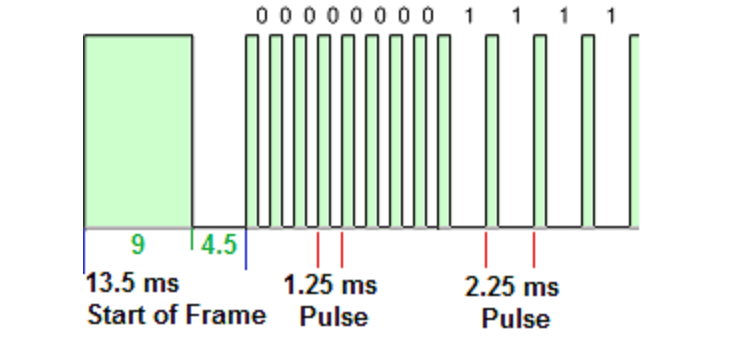
\includegraphics[width=8cm]{images/necOnesAndZeros.png}
   \caption{Wykres elementarnej modulacji sygnału standardu NEC}
   \label{Fig:necOnesZerosFigure}
\end{figure}

Aby wysłać pełne rządanie, które może być interpretowane przez odbiornik, trzeba wysłać informację opatrzoną w pewną strukturę. Najpierw wysyłany jest sygnał rozpoczęcia nadawania. Następnie wysyłany jest 8 bitowy adres urządzenia odbierającego sygnał i kolejno jego negacja bitowa. W takim sam sposób wysyłane jest 8 bitów danych i ich negacja bitowa. Tak zbudowana pojedyncza ramka danych, potrzebuje zawsze 67,5 ms, aby zostać wysłaną, niezależnie od wysyłanych danych i adresu urządzenia dzięki negacji bitowej obu tych segmentów. Przykładowe wysłanie kodu liczbowego 0xAD do urządzenia o adresie 0xFF przedstawione zostało na wykresie znajdującym się na rysunku \ref*{Fig:necFrame}.

\begin{figure}[ht]
   \centering
   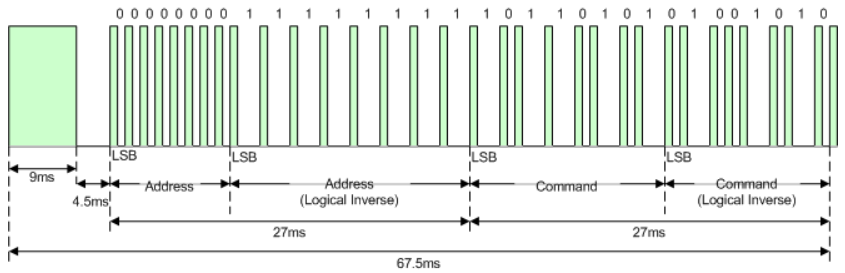
\includegraphics[width=13cm]{images/necFrame.png}
   \caption{Przykładowa modulacja sygnału pełnej wiadomości standardu NEC}
   \label{Fig:necFrame}
\end{figure}

\subsection{System operacyjny Android}
System Android, rozwijany przez firmę Google, stanowi środowisko operacyjne oparte na otwartym kodzie źródłowym. Przyczynia się to do jego wyjątkowej elastyczności i dostosowywalności do różnych urządzeń mobilnych, głównie
smartfonów i tabletów, ale z powodzeniem stosowany jest także w innych urządzeniach przenośnych.

Otwartość kodu umożliwia deweloperom z całego świata dostosowywanie systemu do specyficznych potrzeb. Istotną cechą Androida jest także jego wszechstronność, manifestująca się w szerokiej gamie dostępnych
urządzeń pracujących z tym systemem operacyjnym.
Instalowany jest on na urządzeniach z wszystkich przedziałów cenowych, umożliwiając
programistom tworzenie aplikacji dostępnych dla każdej z grup odbiorców. Sklep Google Play, jako główne źródło
aplikacji, gier, multimediów i innych treści, stanowi istotny element ekosystemu Androida. Ponadto, integracja
z usługami Google, takimi jak Gmail, Google Drive, Google Maps i wielu innych sprawia, że można niemal każdą czynność wykonać przy pomocy dedykowanej aplikacji firmy Google. Względna jednolitość tego środowiska, pomimo takiej gamy obsługiwanych urządzeń sprawia, że dla programistów stanowi ono atrakcyjne pole do
rozwoju i tworzenia innowacyjnych rozwiązań. Platforma jest też bradzo opłacalnym polem biznesowym z uwagi na szeroką bazę użytkowników oraz dynamiczny rynek aplikacji mobilnych. Nie jest więc dziwne, że urządzenia z Androidem posiadało 69,74\% wszytskich użytkowników urzadzeń mobilnych i był on wciąż najczęściej używanym systemem operacyjnym w 2022 roku\cite{androidStats}.
\subsection{Język programowania Dart}
Dart to język programowania stworzony przez Google, zaprojektowany z myślą o tworzeniu wydajnych, skalowalnych i nowoczesnych aplikacji. Jego głównym zastosowaniem jest budowa interaktywnych stron internetowych oraz aplikacji mobilnych przy użyciu zestawu narządzi Flutter.

Język ten charakteryzuje się statycznym typowaniem, co oznacza, że typy zmiennych sprawdzane są w trakcie budowania aplikacji, co może pomóc w wykrywaniu błędów przed uruchomieniem programu. Dart wspiera i opiera się głównie na programowaniu obiektowym.

Jedną z ważnych cech Darta, jest również jego zdolność do wykonywania kodu zarówno w trybie just-in-time (JIT) jak i ahead-of-time (AOT). Tryb JIT umożliwia szybkie rozwijanie i testowanie aplikacji, podczas gdy tryb AOT pozwala na kompilację
kodu źródłowego do natywnego kodu maszynowego, co zwiększa wydajność aplikacji podczas działania. Dart oferuje także mechanizmy asynchroniczne, co jest niezwykle istotne w programowaniu współbieżnym i obsłudze operacji wejścia/wyjścia bez blokowania głównego wątku\cite{dartInfo}.

W kontekście frameworka Flutter, język ten staje się kluczowym narzędziem budowy interfejsów użytkownika. Sam wspomniany zestaw narzędzi został napisany przy pomocy Darta i to z nim najlepiej współpracuje.
\subsection{Framework Flutter}
Flutter to otwartoźródłowy zestaw narzędzi (SDK - Software Development Kit) stworzony przez Google do budowy interfejsów użytkownika (UI - User Inferface). Jest wykorzystywany do tworzenia aplikacji mobilnych, webowych i desktopowych, ze wskazaniem na aplikacje mobilne. Jednym z głównych atutów Fluttera jest możliwość tworzenia jednego kodu źródłowego, który może być budowany do aplikacji dla różnych platform, takich jak Android, iOS, web, Windows czy Linux.

W centrum Fluttera znajduje się Dart, który jest używany do definiowania interfejsu użytkownika oraz logiki biznesowej.
SDK ten bazuje na podejściu deklaratywnym, co oznacza, że w kodzie opisuje się, jak ma wyglądać interfejs w danym momencie, a~nie jak ma być aktualizowany w odpowiedzi na różne zdarzenia. To podejście ułatwia zrozumienie i utrzymanie kodu.
Wprowadza on również własny silnik renderujący. Dzięki temu, dobrze zaprojektowane aplikacje Fluttera charakteryzują się płynnością i~responsywnością.

Zestaw oferuje bogatą gamę wbudowanych widgetów, które są podstawowymi elementami budującymi interfejs użytkownika. Programiści mogą również tworzyć własne niestandardowe widgety, co umożliwia pełną swobodę w projektowaniu UI.

Flutter wspiera hot-reloading, co pozwala na natychmiastowe obserwowanie zmian wprowadzanych w kodzie bez konieczności ponownego uruchamiania całej aplikacji. Korzystanie z tego mechanizmu znacznie skraca się czas pracy podczas rozwijania projektu.
Dzięki narzędziom takim jak Flutter DevTools, umożliwiony jest dostęp do zaawansowanych narzędzi do analizy, debugowania i optymalizacji aplikacji końcowej.\cite{flutterDocs}

Framework ten stał się niebywale popularny wśród programistów. Chcąc tworzyć estetyczne, responsywne i wieloplatformowe aplikacje z minimalnym nakładem pracy, mając do dyspozycji obszerną i interaktywną dokumnetację, jednym z najlepszych wyborów jest wybranie Fluttera jako główne nardzędzie tworzenia interfejsu użytkownika.
\subsection{Komunikacja przez Bluetooth Low Energy}
Bluetooth Low Energy(BLE) to technologia komunikacyjna zaprojektowana do efektywnej wymiany danych pomiędzy urządzeniami przy niskim zużyciu energii. Jest uproszczoną i zoptymalizowaną wersją klasycznego Bluetooth.
Komunikacja za pomocą BLE opiera się na koncepcji dwóch głównych typów urządzeń: urządzenia peryferyjnego i centralnego. Urządzenie peryferyjne emituje dane, podczas gdy urządzenie centralne zbiera te dane.\cite{ble}

Cechą charakterystyczną BLE jest niskie zużycie energii, co sprawia, że jest idealny do zastosowań, gdzie ważne jest przedłużenie życia baterii w urządzeniach przenośnych. Komunikacja BLE opiera się na transmisji krótkich pakietów danych, co przyczynia się do wysokiej efektywności energetycznej.

Usługi w BLE to logiczne grupy charakterystyk, które reprezentowane są jako zestawy danych, udostępniające funkcjonalności lub zestawy operacji odpowiednie dla danej grupy. Charakterystyki z kolei to konkretne funkcje lub dane w ramach danej usługi. GATT (Generic Attribute Profile) jest z kolei protokołem używanym w BLE do opisu i komunikacji z usługami i charakterystykami poprzez klienta GATT. Każda usługa i charakterystyka posiada swój numer UUID.

Komunikacja między urządzeniem centralnym, a peryferyjnym, opiera się na zestawie reguł znanych jako GATT Server (na urządzeniu peryferyjnym) i GATT Client (na urządzeniu centralnym). GATT Server udostępnia usługi i charakterystyki, natomiast GATT Client korzysta z protokołu GATT do odczytywania i zapisywania danych.

Wiele bibliotek na rożne platformy sprzętowe umożliwia łatwe i szybkie obsługiwianie technologii Bluetooth Low Energy przez wydzielenie na wysokim poziomie abstrakcji funkcji, obiektów i metod zdecydowanie ułatwiających korzystanie z~tej technologii. Takie podejście zwalnia z programisty obowiązek zajęcia się niuansami w~projektach, w których nie są one krytycznymi elementami rozwiązania i pozwala na uniknięcie trudnych do zdiagnozowania błędów konfiguracji.

\clearpage

\section{Urządzenie wysyłające sygnały IR}
\subsection{Schemat elektryczny zaprojektowanego urządzenia}
Aby wykonać urzadzenie pośredniczące najpierw wykonano shemat elektryczny przy pomocy programu EasyEDA w darmowej wersji online\cite{easyEda}. Dzięki bibliotekom tworzonym przez użytkowników odnaleziono wszystkie niezbędne elementy do działania urządzenia pośredniczącego. Utworzony schemat elektryczny powstały z użytych komponentów znajduje się na rysunku \ref*{Fig:deviceScheme}.
\begin{figure}[ht]
   \centering
   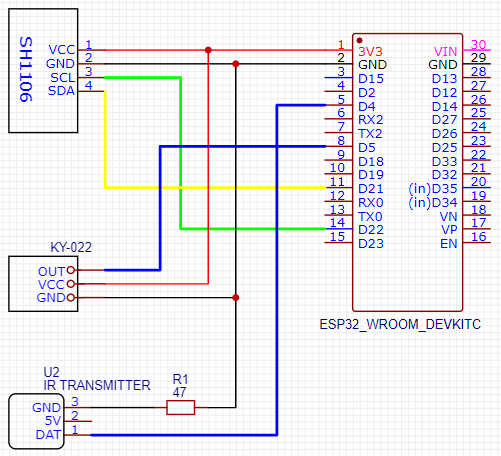
\includegraphics[width=12cm]{images/deviceScheme.png}
   \caption{Schemat elektryczny urządzenia pośredniczącego}
   \label{Fig:deviceScheme}
\end{figure}

Na schemacie kolorem czarnym oznaczono połączenia do masy (GND), kolorem czerwonym zasilanie z mikrokontrolera o potencjale 3.3 V. Na niebiesko zaznaczone są szyny danych modułów IR. Z kolei kolorem zielonym oznaczono linię zegarową, a~żółtym linię danych, porotokołu komunikacjynego I2C wyświetlacza OLED.

Samo urządznie nie jest wrażliwe na zakłócenia elektromagnetyczne, ani nie wymagało ochronnej obudowy do przestestowania poprawności założeń projektowych oraz końcowych testów pełnego systemu, dlatego jako element łączący moduły została użyta płytka stykowa. Dzięki użyciu płytki zachowano pełną funkcjonalność urządzenia oraz zyskano dowolność zmian podczas projektowania rozmieszczenia i połączenia komponentów. Urządznie osadzone na płytce prototypowej zostało przedstawione na rysunku \ref*{Fig:deviceOnBoard}.
\begin{figure}[ht]
   \centering
   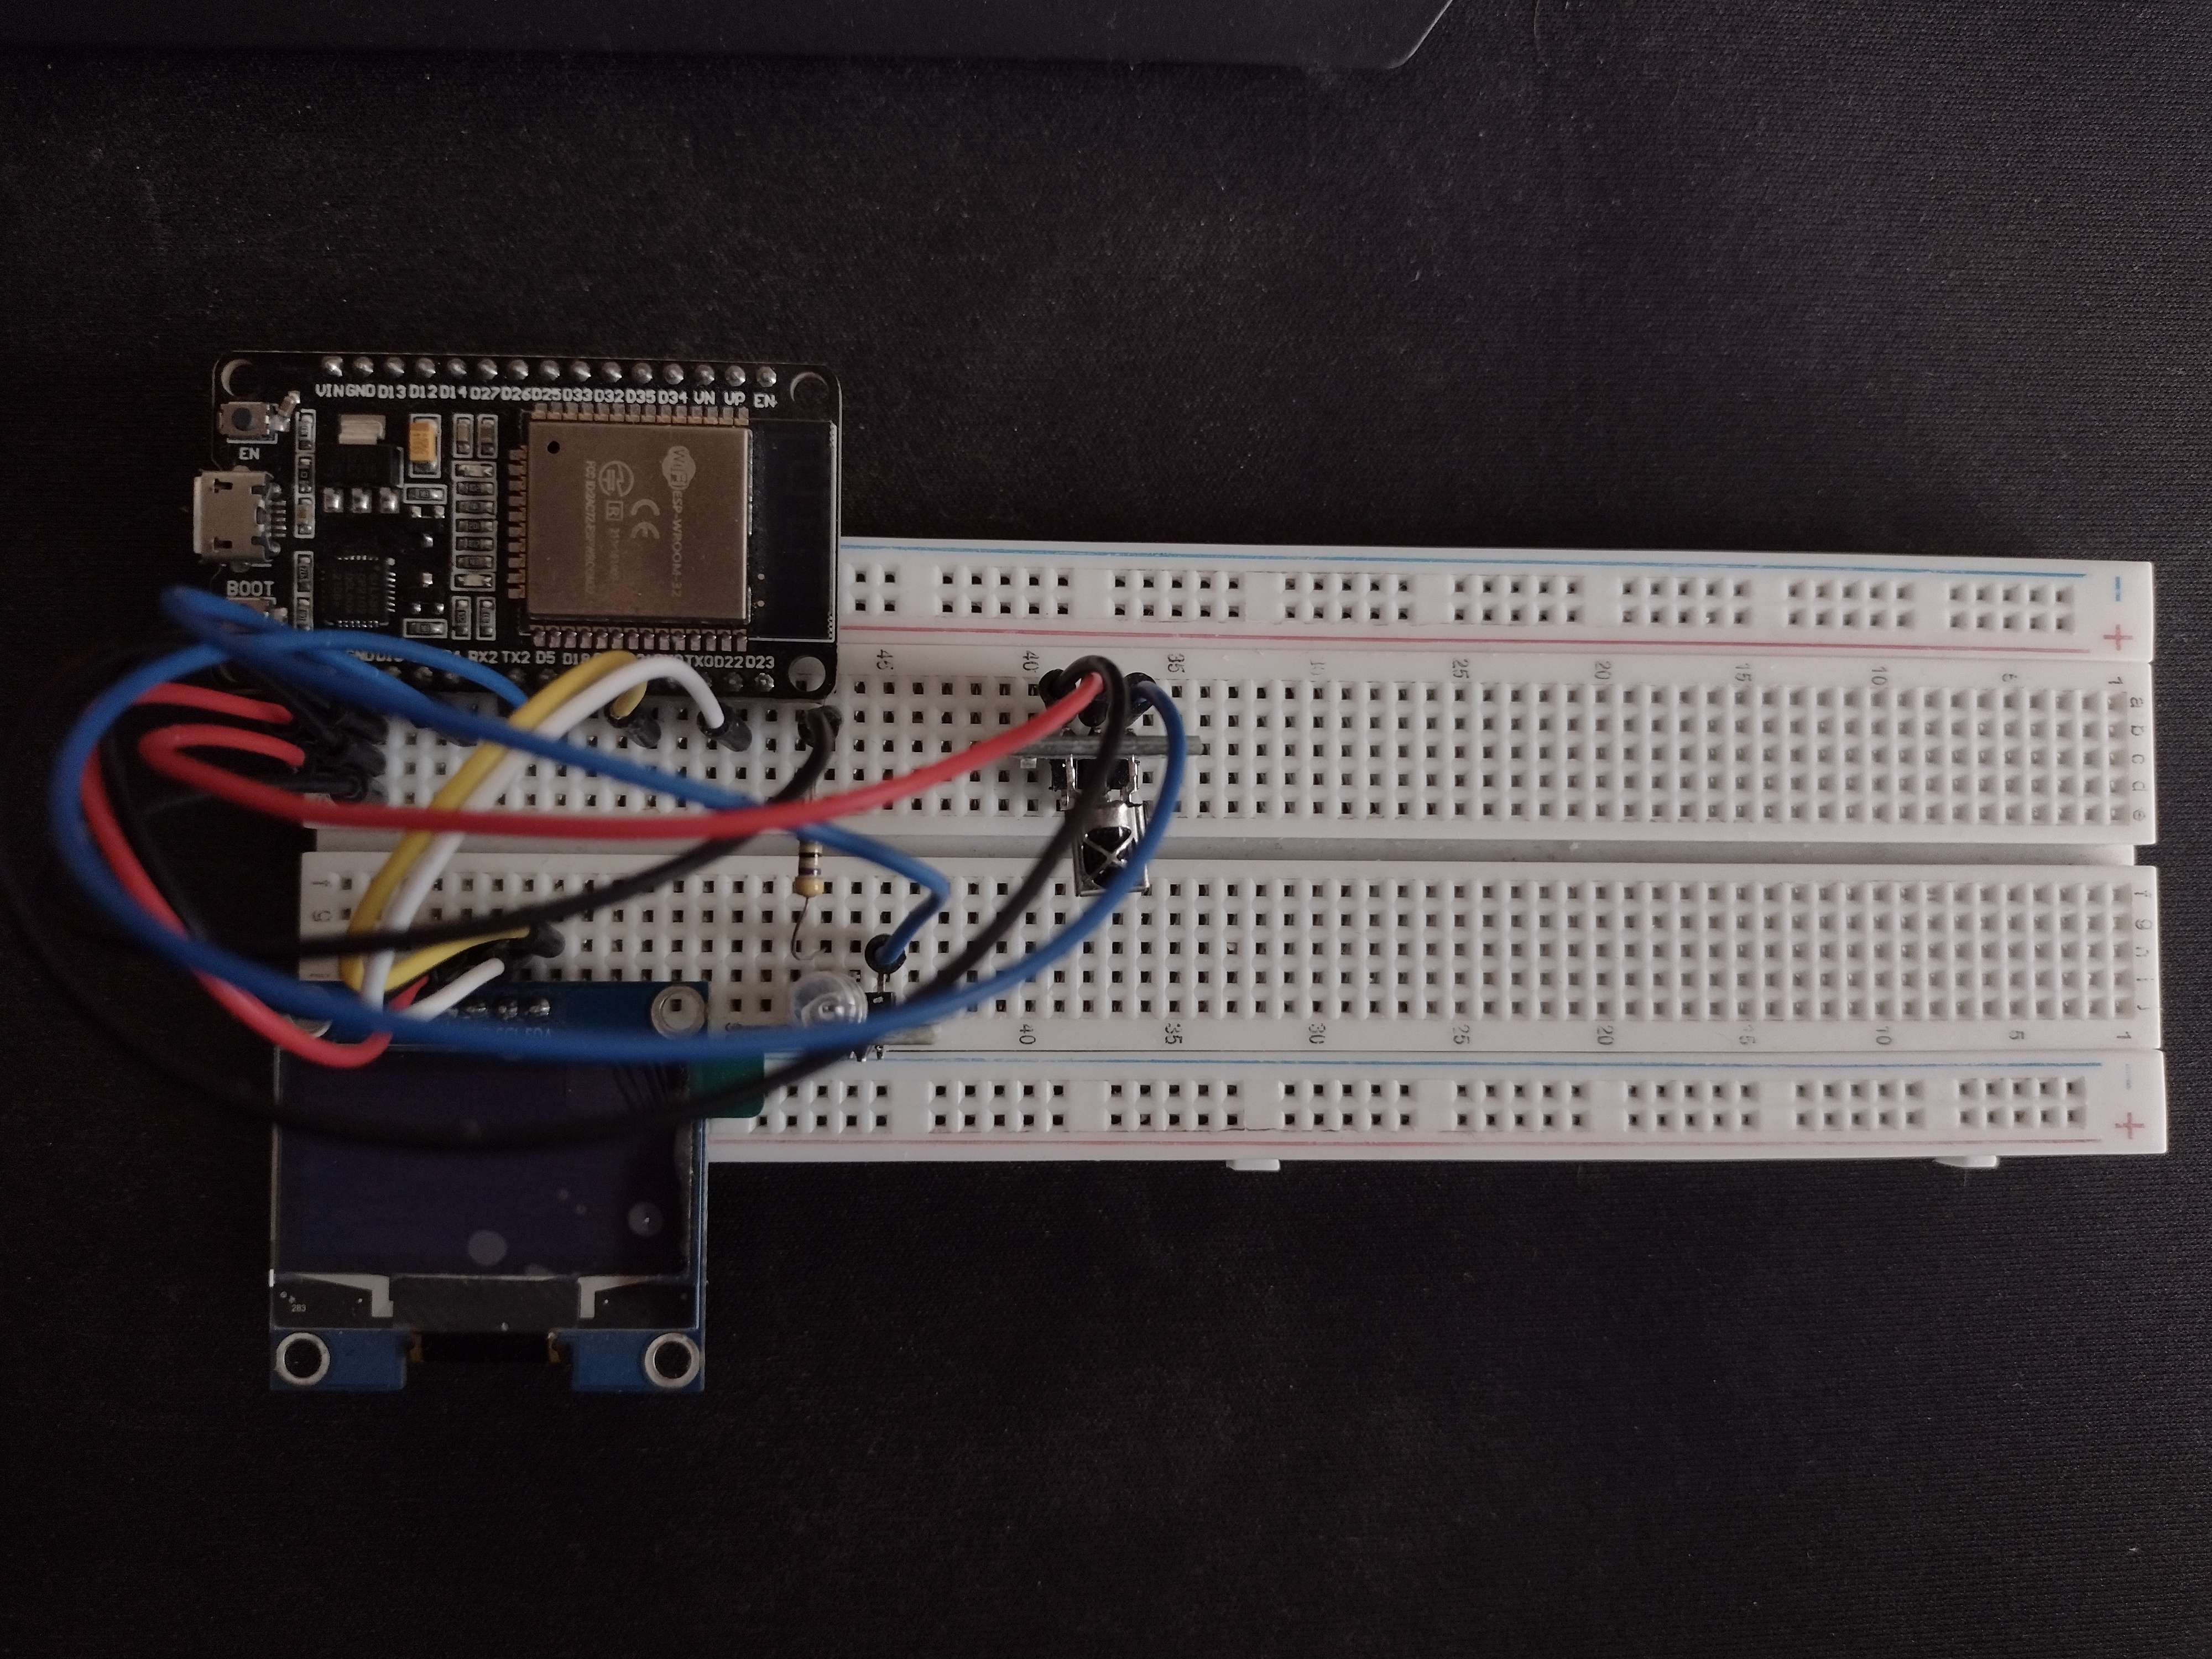
\includegraphics[width=12cm]{images/deviceOnBoard.jpg}
   \caption{Urządzenie pośredniczące osadzone na płytce prototypowej}
   \label{Fig:deviceOnBoard}
\end{figure}
\subsection{Przeglad i opis uzytych komponentow}
Elementy przedstawione na schemacie elektrycznym znalazły się w przedstawionym wcześniej modelu modelu fizycznym. Są to:
\begin{enumerate}[label=\alph*), leftmargin=1.25cm]
   \item Zestaw deweloperski ESP32 Wroom DevKitC V1\cite{doitDevKitV1} -- to system z mikrokontroler ESP32 z procesorem Dual Core Tensilica LX6 240 MHz, pamięcią SRAM 520 KB i pamięcią flash 4 MB. Posiada wbudowane moduły WiFi 802.11 b/g/n oraz moduł Bluetooth Low Energy, dzięki którym nie trzeba dołączać osobnych modułów komunikacji bezprzewodowej. Znajduje się na nim 30 wyprowadzeń GPIO w postaci goldpinów, co znacznie zwiększa wygodę projektowania. Zasilany jest z 5 V ze złącza microUSB lub pinu VCC i GND.
   \item Wyświetlacz OLED SH1106\cite{sh1106} -- to wyświetlacz OLED o przekątnej 1,3'' i rozdzielczości 128 pikseli na 64 pikesle. Ekran oparty jest na sterowniku Adafruit SH1106 pracuje z napięciami 3,3 V oraz 5 V, komunikuje się poprzez protokół I2C. Posiada wlutowane proste złącza goldpin. Wyświetla znaki w kolorze białym.
   \item Transmiter IR KY-005\cite{ky005} -- to moduł nadawczy sygnałów podczerownych. Obsługuje wysyłanie fal IR o długości 940 nm. I pobiera 90 mW mocy podczas działania.
   \item Odbiornik IR KY-022\cite{ky022}  -- to moduł z odbiorczy podczerwieni, działający na częstotliwości 38 kHz. Zasilany jest napięciem od 2,7 V do 5,5 V. Wykrywa sygnał pod maksymalnym kątem odchylenia 90°. Maksymalna odległość wykrywania: 18 m. Posiada cyfrowy sygnał wyjściowy.
   \item Rezystor 47 Ohm -- resystor przewlekany o tolerancji 5 \% i makasymalnej mocy 0,25 W.
   \item Przewody połaczeniowe męsko-męskie.
   \item Płytka stykowa.
\end{enumerate}

\clearpage

\section{Oprogramowanie sterujące urządzeniem wysyłającym sygnały IR}
\subsection{Środowisko narzędziowe}
Kod sterujący urządzeniem pośredniczącym opartym o mikrokontroler ESP32 został przygotowany za pomocą jezyka C++ oraz frameworka Arduino. Cały projekt oprogramowania zarządzany był przez rozszerzenie do edytora tekstu Visual Studio Code czyli PlatformIO, przy pomocy którego, doinstalowywane były też wymagane biblioteki oraz budowany i wgrywany na płytkę ESP32 Wroom DevKitC był program sterujący, a także przeprowadzane debugowanie. Każda z tych operacji mogła się odbyć dzięki wsparciu programowania i debugowania za pomocą portu microUSB, które posiadała płytka oraz rozszerzenie edytora tekstu.
\subsection{Ogólna struktura oprogramowania}
Oprogramowanie sterujące urządzeniem wysyłąjącym sygnały podczerowne zostało podzielone na 4 elementy. Główny z nich to plik \kod{main.cpp} gdzie odbywa się sterowanie urządzeniem, korzystając przy tym z pozostałych modułów. Utworzone zostały 3 moduły narzędziowe, aby główny kod stał się bardziej przejrzysty oraz modularny. Opdowiadają one za obsługę wyświetlacza OLED, komunikację BLE oraz interpretację danych pochodzących z charakterystyk BLE. Wynikowa struktura podziału autorskich elementów oprogramowania została przedstawiona na rysunku \ref*{Fig:codeStructure}.
\begin{figure}[ht]
   \centering
   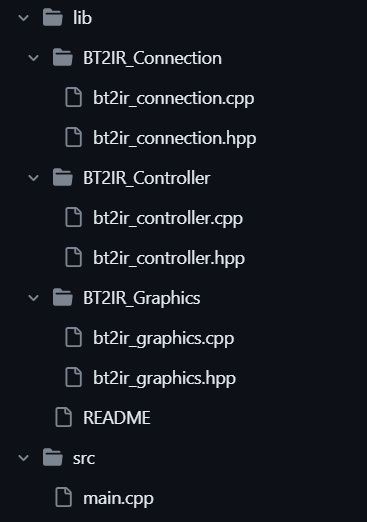
\includegraphics[width=4.5cm]{images/codeStructure.png}
   \caption{Struktura oprogramowania sterującego urządzeniem pośredniczącym}
   \label{Fig:codeStructure}
\end{figure}

\subsection{Główny program sterujący}
Główny program, który steruje całym urządzeniem pośredniczącym znajduje się w~pliku \kod{main.cpp}. Aby zorzumieć jakie funkcjonalności oferuje, najlepiej prześledzić jego budowę.

Najpierw dołączane są pliki nagłówkowe z frameworka Arduino dla ESP32 odpowiadające za obsługę wysyłu i odbioru syngałów podczerwonych. Dołączane są także autorskie moduły z przestrzeni nazw \kod{bt2ir}. Korzystając z nich z kolei można utworzyć globalne obiekty klas, które pozwalają na zarządzanie połączeniem BLE, interpretację danych z charakterystyk tego połączenia, i pracę z  wyświetlaczem OLED. Obiekty tych klas zostają zinicjowane odpowiednimi danymi, prawidłowymi dla posiadanego sprzętu, jak rozdzielczość ekranu OLED czy numery pinów płytki deweloperskiej, na których będą przesyłane dane z i do modułów IR. Kod realizujący dołączanie plików nagłówkowych oraz inicjalizację obiektów globalnych znajduje się na listingu \ref{Lst:globalDefinitions}.

\lstinputlisting[inputencoding=utf8/cp1250, language={C++}, caption={\protect\input{captions/globalDefinitions.txt}\protect\relax}, label={Lst:globalDefinitions}]{codes/globalDefinitions.cpp}

Framework Arduino oczekuje zedefiniowania funkcji \kod{setup()}, która będzie wykonywana raz podczas uruchomienia urządzenia. Utworzono takową i zawarto w niej już na początku zainicjowanie połaczenia szeregowego, aby móc odczytywać dane z~urządzenia, na wypadek chęci wykrycia błędów działania. Znalazła się tam także inicjacja połaczenia z wyświetlaczem OLED poprzez protokół I2C oraz inicjacja serwera BLE, obie inicjacje zostały przeprowadzone za pomocą metod obiektów klas z autorskich modułów. Rozpoczęto w tej funkcji już nasłuchiwanie sygnałów podczerwonych i zainicjowano pracę modułu wysyłającego sygnały IR przy pomocy wcześniej utworzonych obiektów. Zawartość funkcji \kod{setup()} przedstawia kod źródłówy na listingu \ref*{Lst:setup}.

\lstinputlisting[inputencoding=utf8/cp1250, language={C++}, caption={\protect\input{captions/setup.txt}\protect\relax}, label={Lst:setup}]{codes/setup.cpp}

Tworząc oprogramowanie za pomocą frameworka Arduino zdefiniować należy także funkcję, która będzie wykonywana w nieskończonej pętli na programowanym urządzeniu. Narzędzie wymaga nazywała się ona \kod{loop()}. Przed nią jednak znalazły się jeszcze inicjalizacje dwóch znaczników czasowych w postaci dodatnich liczb całkowitych, które zostaną użyte do odliczania czasu trwania wyświetlania komunikatów dla użytkownika.

\begin{figure}[!ht]
\lstinputlisting[inputencoding=utf8/cp1250, language={C++}, caption={\protect\input{captions/loop1.txt}\protect\relax}, label={Lst:loop1}]{codes/loop1.cpp}  
\end{figure}

W samej już funkcji umieszczono instrukcje warunkowe, przez które, sprawdzane jest czy wstąpiły zdarzenia, takie jak: odebranie danych za pomocą serwera BLE o wciśniętym klawiszu w aplikacji, odebranie sygnału podczerwonego na module odbiornika IR, czy też rozłączenie lub połączenie z serwerem BLE nowego użytkownika aplikacji mobilnej. Jeśli program wykryje zdarzenie serwera BLE, rysuje na wyświetlaczu OLED odświeżony stan połaczenia zwierający informację o liczbie połączonych użytkowników. Jeśli z kolei wykryte zostanie zdarzenie odebrania na serwerze BLE informacji o typie wciśniętego przycisku, rysowana jest jego ikona i nazwa, aby poinformować użytkownika o~otrzymaniu jego żądania. Po obsłużeniu zdarzenia resetowana jest flaga informująca o~jego aktywności. Obsługa opisanych zdarzeń w pierwszej części funkcji \kod{loop()} została przedstawiona na listingu \ref*{Lst:loop1}.


\begin{figure}[!ht]
\lstinputlisting[inputencoding=utf8/cp1250, language={C++}, caption={\protect\input{captions/loop2.txt}\protect\relax}, label={Lst:loop2}]{codes/loop2.cpp}
\end{figure}

Program reaguje też na otrzymanie szesnastkowego kodu IR po wciśnieciu przycisku  pilota w aplikacji mobilnej. Po otrzymaniu tego kodu przez BLE, przesyłany jest on dalej w formie sygnału podczerwonego do telewizora, realizując w ten sposób sterowanie nim, po zakończeniu już obsługi zdarzenia resetowana jest jego flaga. Jeżeli odczytany zostanie na zewnętrznym module odbiorczym, prawidłowy sygnał podczerwony, wypisany zostaje on na wyświetlaczu OLED, dzięki dedykowanej metodzie obiektu sterującego tym ekranem. Aktualizowany zostaje też wtedy znacznik czasowy tego zdarzenia. Następnie też wznawiane jest nasłuchiwanie sygnałów podczerwonych. Każdy z komunikatów dla użytkownika posiada swój czas wyświetlania. Limitowanie czasu ich trwania jest realizowane za pomocą sprawdzania stempli czasowych. Jeśli któryś z komunikatów powinien już się zakończyć, co jest wnioskowane na podstawie odległości aktualnego czasu od odpowiedniego znacznika czasowego, resetowane są wszystkie znaczniki czasowe komunikatów i następuje wyświetlenie domyślnego ekranu stanu połączenia BLE. Te funkcjonalności znalazły się w drugiej części funkcji \kod{loop()}, a jej kod źródłowy został przedstawiony na listingu \ref{Lst:loop2}.



\subsection{Moduł komunikacji poprzez BLE}
Autorski moduł odpowiedzialny za komunikację BLE został oparty o moduły biblioteki NimBLE\cite{nimBLE}, zamiast podstawowej biblioteki przygotowanej przez Arduino, ponieważ ta druga zajmowała zbyt wiele miejsca w pamięci FLASH mikrokontrolera. Wszystkie elementy tego modułu znalazły się w przestrzeni nazw \kod{bt2ir}.

Klasa zarządzająca połaczeniem BLE została utworzona przy pomocy wzorca projektowego Singleton\cite{designPatterns}, który powoduje że użytkownich korzysta z logicznie tylko jednej instancji takiej klasy, przechowywanej pomiędzy obiektami za pomocą uchywtu, którym dla języka C++ stał się wskaźnik. Zasosowano ten wzorzec aby zachowywać informacje o połączeniu BLE w całym programie i modduły mogły korzystać jednocześnie z tego samego połącznia w wygodny sposób. Publiczne funkcjonalności tej klasy udostępnione za pomocą metod to:
\begin{enumerate}[label=\alph*), leftmargin=1.25cm]
   \item inicjalizacja serwera BLE
   \item możliwość odczytywania i edytowania liczby połączonych urządzeń
   \item możliwość odczytywania i edytowania flag zdarzeń odebrania danych wciśniętego przycisku w aplikacji mobilnej
   \item dostęp do charakterystyk odebranego typu przycisku i jego kodu IR
   \item metoda pozwalająca narysować aktualny stan połączenia BLE.
\end{enumerate} Część pliku nagłówkowego zawierająca dostępne metody publiczne klasy \kod{Connection} została przedstawiona na listingu \ref*{Lst:bleMethods}.

\lstinputlisting[inputencoding=utf8/cp1250, language={C++}, caption={\protect\input{captions/bleMethods.txt}\protect\relax}, label={Lst:bleMethods}]{codes/bleMethods.cpp}

Najważniejszym elementem tego modułu jest metoda \kod{setupConnection()} klasy \kod{Connection}. W niej właśnie odbywa się inicjowanie serwera BLE wraz z jego parametrami oraz dołączenie funkcji wywoływanych podczas zdarzeń serwera.

Podczas przygotowywania urządzenia pośredniczącego do obsługi BLE w pierwszej kolejności inicjowane jest abstrakcja urządzenia. Kolejno dalej na urządzeniu tworzony jest serwer i przypisywane są mu autorskie klasy przechowujące metody wywoływane przez zdarzenia serwera, zawarte także w tym module, dzięki czemu biblioteka automatycznie będzie wykonywać czynności po połączeniu i rozłączeniu użytkownika, oraz o takim wydarzeniu zostanie poinformowany główny program sterujący.
Na tak utworzonym serwerze tworzony jest serwis i jego 2 charakterystyki odpowiadające wyłącznie za odbieranie danych o typie wciśniętego przycisku i jego szesnastkowym kodzie IR. Obie charakterystyki otrzymują także swoje klasy z metodami wywoływanymi podczas odebrania danych, dzięki czemu główny program sterujący informowany jest o tym zdarzeniu. Utworzony w ten sposób serwer może rozpocząć rozgłaszanie swojej obecności i nazwiązywać połączenia z klientami. Kod funkcji realizującej inicjalizację serwera BLE znajduje się na listingu \ref*{Lst:setupConnection}.

\lstinputlisting[inputencoding=utf8/cp1250, language={C++}, caption={\protect\input{captions/setupConnection.txt}\protect\relax}, label={Lst:setupConnection}]{codes/setupConnection.cpp}

Aby uzyskać możliwość połaczenia wielu użytkowników z serwerem BLE urządzenia pośredniczącego metoda wywoływana podczas każdego połączenia nowego użytkownika musi wznowić rozgłaszanie dostępności serwera. Ta funkcjonalność została zaimplementowana w funkcjach wywwoływanych podczas zdarzeń serwera.
\subsection{Moduł interpretujący dane z serwera BLE}
Aby ułatwić pracę z danymi odebranymi przez urządznie pośredniczące utworzono moduł przetwarzający je. Zawiera on wygodny typ wylieczniowy wykorzystywany do nadawania przejrzystych nazw programowych dla odebranych typów wciśniętego przycisku pilota z aplikacji mobilnej.
Z kolei klasa \kod{Controller} odpowiada za interpretację danych, odebranych za pomocą charakterystyk serwera BLE. Korzysta ona z instancji klasy \kod{Connection} aby pobrać dane z charakterystyk i je przetworzyć. W~tym celu, klasa ta, udostępnia metody pozwalające odświeżać przechowywane jej polach prywatnych ostatnio odebrane dane od aplikacji mobilnej. Publicznie dostępne elementy modułu znajdują się na listingu \ref*{Lst:controller}.
\vfill

\lstinputlisting[inputencoding=utf8/cp1250, language={C++}, caption={\protect\input{captions/controller.txt}\protect\relax}, label={Lst:controller}]{codes/controller.cpp}

Dane odebrane za pomocą charakterystyk przechowywane są w postaci bitowej. Aby odczytać ich wartości należy zinterpretować ich zawartość za pomocą odpowiedniego szablonu, który w tym przypadku będzie typem danych. Metoda \kod{updateButton\-Type()} z klasy \kod{Controller} interpretuje dane charakterystki za pomocą typu 8~bitowej liczby całkowitej bez znaku, ponieważ ilość przycisków jest niewielka. Odbywa się tam też prosta kontrola poprawności danych, poprzez sprawdzenie czy odebrane dane mieszczą się w zakresie zdefiniowanych przycisków pilota. Kod źródłowy tej funkcji znajduje się na listingu \ref*{Lst:dataProcessing}.

\lstinputlisting[inputencoding=utf8/cp1250, language={C++}, caption={\protect\input{captions/dataProcessing.txt}\protect\relax}, label={Lst:dataProcessing}]{codes/dataProcessing.cpp}

\subsection{Moduł obsługi ekranu OLED}
Autorski moduł obsługi ekranu OLED jest w rzeczywistości nakładką na klasę sterującą wyświetlaczem OLED z bibliotek firmy Adafruit. Taka relacja realizowania jest za pomocą dziedziczenia publicznego po klasie \kod{Adafruit\_SH1106G} w utworzonej klasie nakładki \kod{Display}. Sama nakładka znalazła się w przestrzeni nazw \kod{bt2ir}.

Utworzona klasa nakładki stara się udostępnić metody, dzięki którym użytkownik w prosty i przejrzysty sposób może rysować konkretne obrazy i napisy na wyświetlaczu, w postaci przygotowanych i zparametryzowanych ekranów. Udostępnione zostały ekrany takie jak przedstawienie liczby połączonych smartfonów z serwerem BLE i jego stanu, wyświetlanie komunikatu o odebraniu wciśniętego przycisku z aplikacji mobilnej, czy wyświetlenia odebranego za pomocą modułu odbiorczego z diodą sygnału IR. Lista dostępnych funkcjonalności utworzonej nakładki w postaci metod publicznych została przedstawiona na listingu \ref*{Lst:graphics}.

\lstinputlisting[inputencoding=utf8/cp1250, language={C++}, caption={\protect\input{captions/graphics.txt}\protect\relax}, label={Lst:graphics}]{codes/graphics.cpp}

Ukryta dla użtykownika logika tej nakładki opiera się o 4 metody prywatne. Dwie z nich rysują bardziej podstawowe elementy ekranów, takie jak rysowanie wyrównanego tekstu czy wielkich cyfr. Dzięki nim powstały także dwie metody z nich korzystające, przy pomocy których, można narysować na wyświetlaczu ikonę z podpisem lub cyfrę z podpisem. Tak wydzielone fragmenty logiki kodu, przyspieszyły i~ułatwiły zbudowanie wszystkich publicznie dostępnych funkcjonalności. Utworzona lista prywatnych metod zaprojektowanej klasy znajduje się na listingu \ref*{Lst:graphicsPrivate}.

\lstinputlisting[inputencoding=utf8/cp1250, language={C++}, caption={\protect\input{captions/graphicsPrivate.txt}\protect\relax}, label={Lst:graphicsPrivate}]{codes/graphicsPrivate.cpp}

Ikony rysowane na ekranach przez publiczne metody nakładki zostały umieszczone w programie za pomocą tablic bajtów, a same tablice zostały wygenerowane poprzez progowanie binarne obrazów w odcieniach szarości, przy pomocy aplikacji internetowej image2cpp\cite{image2cpp}. Po przekonwertowaniu obrazów na tablice bajtów i usunięciu z~jej otoczenia niepotrzebnie wygenerowanych części kodu, można ją umieścić w oprogramowaniu i wykorzystywać do wyświetlania obrazu, którego ta tablica dotyczy. Jedna z~wygenerowanych tablic znajduje się na listingu \ref*{Lst:imageArray}.
\vfill

\lstinputlisting[inputencoding=utf8/cp1250, language={C++}, caption={\protect\input{captions/imageArray.txt}\protect\relax}, label={Lst:imageArray}]{codes/imageArray.cpp}

Dzięki utworzonym narzędziom budowano publiczne metody dostępne dla użytkownika nakładki. W każdej takiej funkcji najpierw czyszczony był wyświetlacz, następnie rysowano w buforze ekranu odpowiedni obraz na podstawie zdefiniowanych tablic bajtów wraz z wyśrodkowanym podpisem, by końcowo wyświetlić dane zgromadzone w~buforze rysowania. Jedną z tych metod jest \kod{drawMoveUp()} rysująca komunikat dla użytkownika o wciśnięciu przycisku przejścia w górę na pilocie w aplikacji mobilnej. Jej implementacja została przedstawiona na listingu \ref*{Lst:drawMoveUp}, a jej fizyczny efekt na wyświetlaczu OLED pokazano na rysunku \ref*{Fig:drawMoveUp}.

\lstinputlisting[inputencoding=utf8/cp1250, language={C++}, caption={\protect\input{captions/drawMoveUp.txt}\protect\relax}, label={Lst:drawMoveUp}]{codes/drawMoveUp.cpp}

Więcej ekranów i obrazów, które może przedstawiać wyświetlacz OLED osadzony w urządzeniu pośredniczącym zostały zawarte w prezentacji pełnego systemu. W ten sposób opatrzone są w odpowiedni konekst ułatwiający zrozumienie ich celowości.

\begin{figure}[ht]
   \centering
   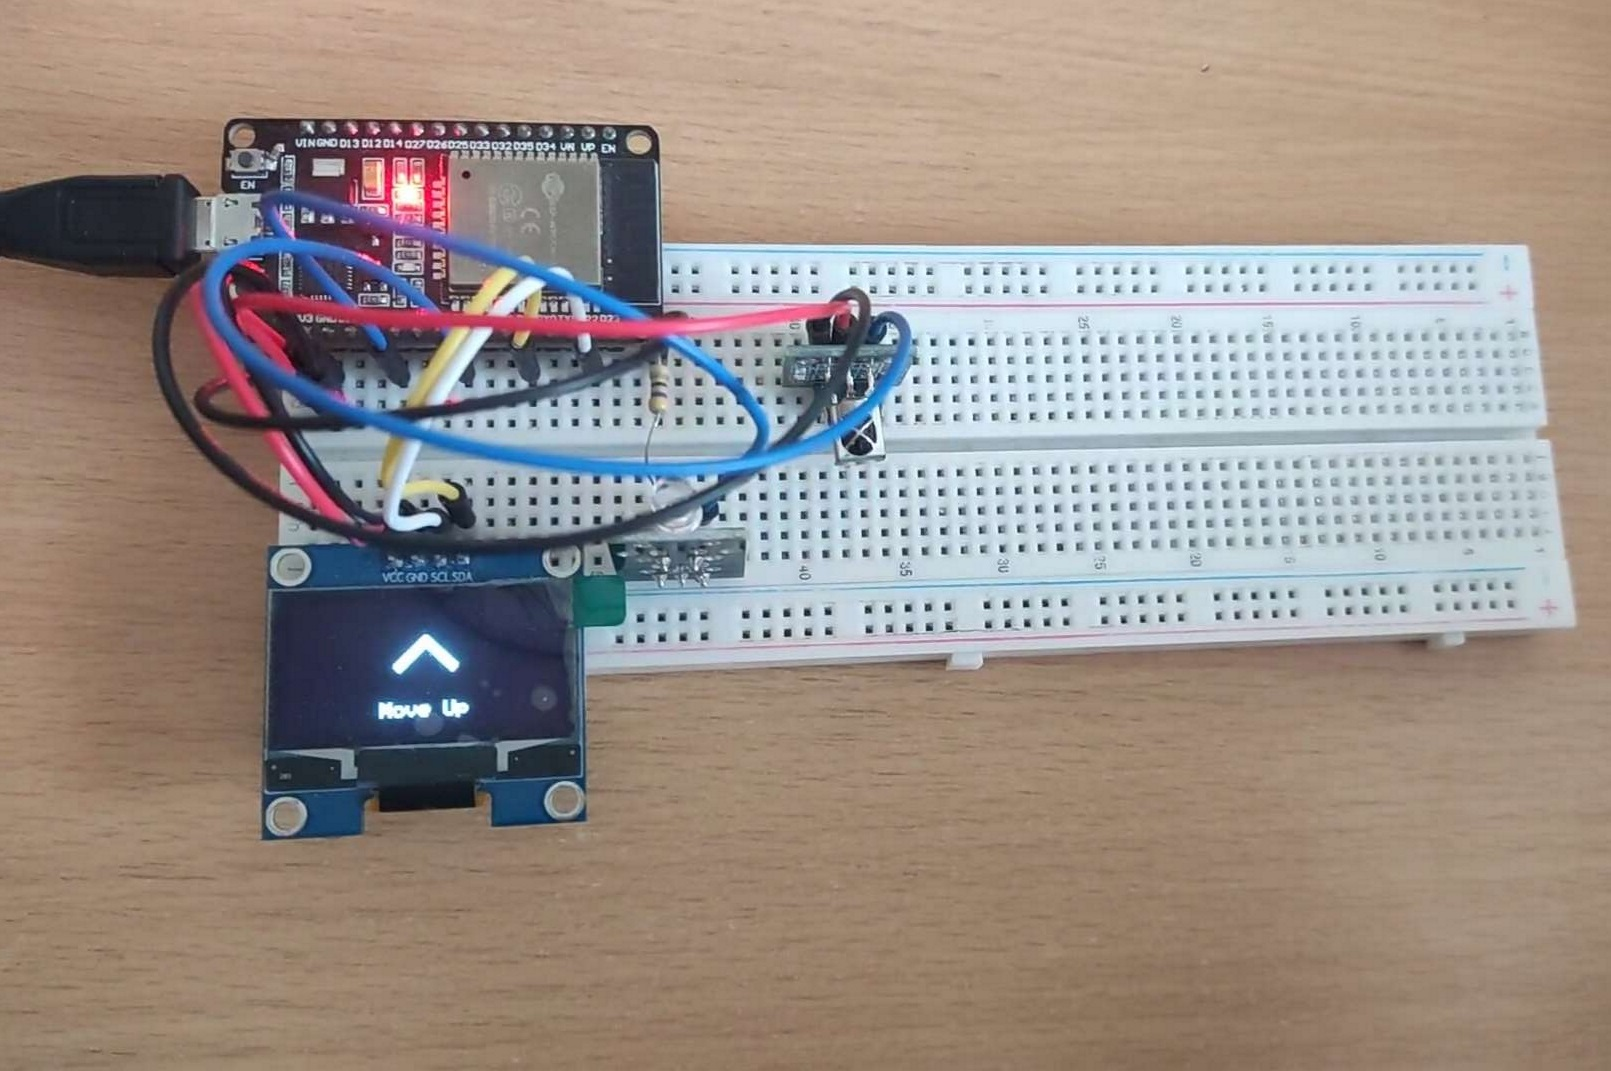
\includegraphics[width=14cm]{images/drawMoveUp.jpg}
   \caption{Wynik wywołania metody rysującej strzałkę w górę z opisem na wyświetlaczu}
   \label{Fig:drawMoveUp}
\end{figure}

\clearpage

\section{Zakończenie}

Niniejsza praca miała na celu zaproponowanie rozwiązania sterowania telewizorem z poziomu smartfona dzięki aplikacji mobilnej i urządzeniu pośredniczącym opartemu o mikrokontroler z niezbędnymi modułami. Omówiono w niej technologie i~koncepty, z których korzystano podczas procesu projektowania tego systemu. Opisane zostały też najważniejsze elementy fizycznej części projektu, oprogramowanie mikrokontrolera, zbudowana aplikacja mobilna oraz ich współpraca w cely sterowania telewizorem.

Utworzony prototyp systemu zapewnił możliwość programowania przycisków pilota w aplikacji mobilnej w oparciu o szesnastkowe kody sygnałów podczerwonych. Kody te można uzyskać przeglądając sieć i strony producentów urządzeń multimedialnych oraz dzięki wbudowanemu w urządzenie pośredniczące czytnikowi kodów IR, który po odebraniu takiego kodu przez podczerwień, wyświetla go na ekranie OLED. Przy pomocy serwera BLE zastosowanego na urządzeniu wysyłającym sygnały podczerwone zapewniono także dostęp do systemu dla wielu użytkowników jednocześnie. Utworzona aplikacja mobilna jest prosta w użytkowaniu i intuicyjna nawet dla użytkowników nieobytych z technologią obecną w dzisiejszych smartfonach, a duże i wyraziste elementy pozwalają się dostrzec nawet z większych odległości.

Zaprojektowany prototypowy system aplikacji mobilnej i urządzenia pośredniczącego opartego o mikrokontroler jest już w pełni funkcjonalny i może nawet zostać przekształcony do produktu komercyjnego. Aby zwiększyć jednak atrakcyjność tego rozwiązania na rynku, można wskazać kilka usprawnień jak na przykład:
\begin{itemize}[label=-,labelsep=0.4cm,leftmargin=0.65cm]
   \item zamknięcie urządzenia pośredniczącego w wygodnej prostokątnej obudowie z odpowiednim rozłożeniem modułów,
   \item wprowadznie automatyzacji programowania kodów IR i wczytywania ich z plików JSON, udostępnianych też na stronie internetowej firmy,
   \item dodanie obsługi inteligentnych gestów użytkownika w aplikacji dla konkretnych typów urządzeń,
   \item wprowadzenie kreatora ekranów przycisków pilota w aplikacji dla maksymalnej uniwersalności rozwiązania,
   \item wprowadzenie systemu logowania, aby przechowywać zestawy przycisków na serwerze, dzięki czemu będą one dostępne dla wielu urządzeń tego użytkownika
   
\end{itemize}

Autor za własny wkład pracy uważa: 
\begin{itemize}[label=-,labelsep=0.4cm,leftmargin=0.65cm]
   \item przegląd i dobór technologii do utworzonego rozwiązania,
   \item zaprojektowanie urządzenia pośredniczącego opartego o mikrokontroler wysyłającego i odbierającego sygnały IR,
   \item zaprojektowanie interfejsu użytkownika aplikacji mobilnej,
   \item zaprojektowanie komunikacji aplikacji mobilnej pilota uniwersalnego z mikrokontrolerem w oparciu o~technologię BLE,
   \item utworzenie odpowiedniego oprogramowania sterującego dla mikrokontrolera,
   \item zbudowanie i oprogramowanie aplikacji mobilnej,
   \item opis oprogramowania i przedstawienie elementów utworzonego systemu.
   
\end{itemize}

\clearpage
\addcontentsline{toc}{section}{Literatura}
\bibliography{biblgr}
\bibliographystyle{plain}

\clearpage

\makesummary

\end{document}
